\section{Workflow}
	\begin{enumerate}
	\item User submits a witness
	\item Verification: did the user send a digitization?
	\item A flash message informs the user of the delay for receiving the annotations
	\item Images are downloaded and \iiif manifest is generated
	\item POST request is sent from \eida to \exapi with manifest link and type of witness as parameters
	\item \api: images are downloaded, detection is launched and annotation file is generated
	\item POST request is sent from \exapi to \eida with annotation file
	\item Annotations are indexed to be displayed for the user
	\end{enumerate}

\section{Settings}
	\subsection{EiDA}
	In the \texttt{.env} file, the \texttt{EXAPI} variable must be set with the \URL of the \api.
	\begin{lstlisting}
		EXAPI="<gpu-api-address>"\end{lstlisting}
	
	In the settings file \texttt{settings.py}, complete the \texttt{GPU\_PORT} variable so the \texttt{GPU\_URL} variable can be set.
	\begin{lstlisting}
		GPU_PORT = 5000
		GPU_URL = f"{ENV('EXAPI')}:{GPU_PORT}"\end{lstlisting}

	\subsection{extractorAPI}
	In the \texttt{.env} file, set the \texttt{CLIENT\_APP\_URL} variable with the \URL of the app.
	\begin{lstlisting}
		CLIENT_APP_URL="<url>"\end{lstlisting}

\section{Sending for detection}
	\begin{figure}[h]
	\centering
	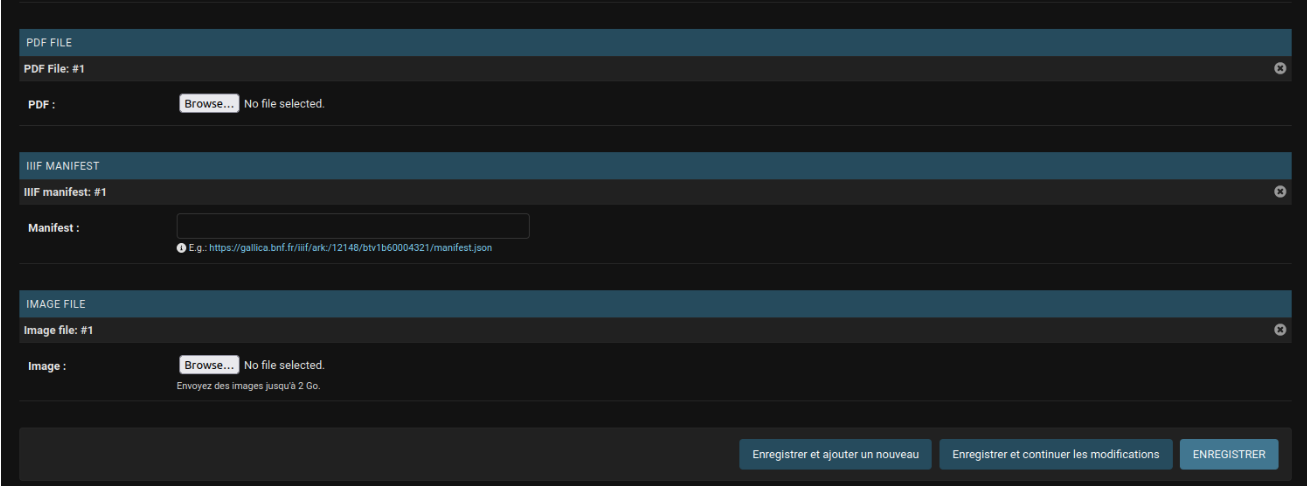
\includegraphics[width=15cm]{images/eida_send_manifest.png}
	\caption{Capture d'écran du formulaire d'envoi d'une numérisation dans l'application \eida}
	\label{fig:eida_send_manifest}
	\end{figure}

	\subsection{IIIF manifest}
	The user creates a \textbf{witness}, fills in the form and submit a digitization (either a PDF file, a \iiif manifest or images).

	The images are downloaded and the \textbf{\eida \iiif manifest} is generated: the request to the \api is not sent until all of the images are downloaded, to avoid errors and annotation of incomplete manifests.

	\subsection{annotate\_wit function}
	To send requests to \exapi from the \eida application, we created a function in \texttt{vhs-platform/vhsapp/utils/iiif/annotation.py}. The function sends a \textbf{POST request} to the \api endpoint \texttt{/run\_detect}, which launches detection on the images from the digitization.
	
	The request takes as arguments the \textbf{\URL of the manifest} we want annotated, and the \textbf{abbreviation} of the witness type.
	
	The \texttt{event} argument is used with the method \texttt{.wait()} to ensure the function \textbf{waits for an event to be set} before sending the request to the \api – this event will be set when the images from the previous step are all downloaded.
	
	\begin{lstlisting}[language=Python]
	def annotate_wit(event, witness_id, wit_abbr=MS_ABBR, version=MANIFEST_AUTO):
		wit_type = MS if wit_abbr == MS_ABBR else VOL
		api_endpoint = f"{GPU_URL}/run_detect"
	
		manifest_url = (
			f"{VHS_APP_URL}/{APP_NAME}/iiif/{version}/{wit_type}/{witness_id}/manifest.json"
		)
		data = {"manifest_url": manifest_url, "wit_abbr": wit_abbr}
	
		event.wait()
		requests.post(url=api_endpoint, data=data)
		
		return print(f"Witness {witness_id} sent for diagram extraction")\end{lstlisting}
	
	\subsection{Automating the annotation request}
	To launch annotation automatically after the user submits a digitization, we added a \textbf{background task} to the save method of \texttt{Manifests}, \texttt{Pdf} and \texttt{Image} objects.
	
	We use \textbf{threading} to avoid an interruption of the other tasks of the app while waiting for a response to the request.

		\subsubsection{User submitted a IIIF manifest}
		For manifests, we modified the save method of the \texttt{ManifestManuscript} and the \texttt{ManifestVolume} classes in \texttt{vhs/vhs-platform/vhsapp/models/digitization.py}. Ideally, we would have a unique save method for both types.
		
		An \texttt{event} object is created and can be passed through the various \textbf{threads}: the first thread \texttt{t} calls the function \texttt{extract\_images\_from\_iiif\_manifest} (in \texttt{vhs/vhs-platform/ vhsapp/utils/iiif/download.py}) to download images and \textbf{set the event} when the function is done running.

		\begin{lstlisting}[language=Python]
	def extract_images_from_iiif_manifest(manifest_url, witness_ref, event):
		"""
		Extract all images from an IIIF manifest
		"""
		downloader = IIIFDownloader(manifest_url, witness_ref)
		downloader.run()
		event.set()\end{lstlisting}

		\texttt{event.set()} returns a boolean value: event is \texttt{True} when the function has \textbf{run to its completion}. Because we used an \texttt{event.wait()} in the \texttt{annotate\_wit} function, it cannot run unless this value is \texttt{True}.
		
		When the image extraction is done and the event is set, the thread \texttt{t2} starts, therefore \textbf{sending the newly generated manifest to the \api for annotation}.

		\begin{lstlisting}[language=Python]
	class ManifestManuscript(Manifest):
		manuscript = models.ForeignKey(Manuscript, on_delete=models.CASCADE)
		
		def save(self, *args, **kwargs):
			# Call the parent save method to save the model
			super().save(*args, **kwargs)
			
			event = threading.Event()
		
			# Run the async extraction of images from an IIIF manifest in the background using threading
			t = threading.Thread(
				target=extract_images_from_iiif_manifest,
				args=(
					self.manifest,
					f"{MS_ABBR}{self.manuscript.id}",
					event,
				),
			)
			t.start()
			
			t2 = threading.Thread(
				target=annotate_wit,
				args=(
					event,
					f"{self.manuscript.id}",
					f"{MS_ABBR}",
				),
			)
			t2.start()\end{lstlisting}
	
		\subsubsection{User submitted a PDF file}
		For PDF files, the process is the same as for manifests.
		The \texttt{event} is set at the end of the \texttt{pdf\_to\_img function}, when all pages are converted to images, in \texttt{vhs/vhs-platform/ vhsapp/utils/functions.py}.

		\begin{lstlisting}[language=Python]
	def pdf_to_img(event, pdf_name):
		"""
		Convert the PDF file to JPEG images
		"""
		pdf_path = f"{BASE_DIR}/{MEDIA_PATH}/{pdf_name}"
		
		# e.g. pdf_name = "volumes/pdf/filename.pdf" => "filename"
		pdf_name = pdf_path.split("/")[-1].split(".")[0]
		pdf_info = pdfinfo_from_path(pdf_path, userpw=None, poppler_path=None)
		page_nb = pdf_info["Pages"]
		step = 2
		try:
			for img_nb in range(1, page_nb + 1, step):
				batch_pages = convert_from_path(
				pdf_path,
				dpi=300,
				first_page=img_nb,
				last_page=min(img_nb + step - 1, page_nb),
				)
				for page in batch_pages:
					save_img(page, f"{pdf_name}_{img_nb:04d}.jpg")
					img_nb += 1
			event.set()
		except Exception as e:
			log(f"[pdf_to_img] Failed to convert {pdf_name}.pdf to images:\n{e}")\end{lstlisting}

		In \texttt{vhs/vhs-platform/vhsapp/models/digitization.py}, the \texttt{save} method of the \texttt{Pdf} class was modified to start a second thread when the function has run.
		
		\begin{lstlisting}[language=Python]
	class Pdf(Digitization):
		class Meta:
			verbose_name = "PDF File"
			verbose_name_plural = "PDF Files"
			abstract = True  # TODO: make this class not abstract
		
		def __str__(self):
			return self.pdf.name
		
		def save(self, *args, **kwargs):
			# Call the parent save method to save the model
			super().save(*args, **kwargs)
			# Run the PDF to image async conversion task in the background using threading
			# t = threading.Thread(target=self.to_img())
	
			event = threading.Event()
			
			t = threading.Thread(target=pdf_to_img, args=(event, f"{self.pdf.name}",))
			t.start()
		
			t2 = threading.Thread(
				target=annotate_wit,
				args=(
					event,
					f"{self.volume.id if 'vol' in self.pdf.name else self.manuscript.id}",
					f"{VOL_ABBR if 'vol' in self.pdf.name else MS_ABBR}",
				),
			)
			t2.start()\end{lstlisting}

		\subsubsection{User submitted images}
		\begin{lstlisting}[language=Python]
	def save(self, *args, **kwargs):
		if self.image:
			img = Image.open(self.image)
			# Check if the image format is not JPEG
			if img.format != "JPEG":
				# Convert the image to JPEG format
				self.image = convert_to_jpeg(self.image)
		# Call the parent save method to save the model
		super().save(*args, **kwargs)
		
		event = threading.Event()
	
		t = threading.Thread(
			target=annotate_wit,
			args=(
				event,
				f"{self.volume.id if 'vol' in self.image.name else self.manuscript.id}",
				f"{VOL_ABBR if 'vol' in self.image.name else MS_ABBR}",
			),
		)
		t.start()\end{lstlisting}
		
\section{Receiving annotations}
For the annotations to be returned \textbf{from \exapi to the \eida application} after detection, we create an \textbf{endpoint} in \texttt{vhs/vhs-platform/vhs/urls.py}.

\begin{lstlisting}[language=Python]
	path(
		f"{APP_NAME}/<str:wit_type>/<int:wit_id>/annotate/",
		receive_anno,
		name="receive-annotations",
	),\end{lstlisting}

The endpoint calls the function \texttt{receive\_anno} in \texttt{vhs/vhs-platform/vhsapp/utils/ views.py} which receives a \textbf{file} from a \textbf{POST request from \exapi}. When the file is received, \textbf{if it is a text file}, its content is \textbf{written in a file in the annotation directory}. If the file already exists, the content is rewritten.

When the annotation file is saved, the annotations are indexed by the function \texttt{index\_anno}. 

\begin{lstlisting}[language=Python]
	def receive_anno(request, wit_id, wit_type):
		if request.method == "POST":
			annotation_file = request.FILES["annotation_file"]
			file_content = annotation_file.read()
		
			if is_text_file(file_content):
				anno_path = f"{BASE_DIR}/{MEDIA_PATH}/{MS_ANNO_PATH if wit_type == 'manuscript' else VOL_ANNO_PATH}"
				
				try:
					with open(f"{anno_path}/{wit_id}.txt", "w+b") as f:
						f.write(file_content)
		
				except Exception as e:
					log(f"[receive_anno] Failed to open received annotations for {wit_type} #{wit_id}: {e}")
		
				manifest_url = (f"{VHS_APP_URL}/{APP_NAME}/iiif/v2/{wit_type}/{wit_id}/manifest.json")
				try:
					index_anno(manifest_url, wit_type, wit_id)
				except Exception as e:
					log(f"[receive_anno] Failed to index annotations for {wit_type} #{wit_id}: {e}")
					
				return JsonResponse({"message": "Annotation received and indexed."})
			else:
				return JsonResponse({"message": "Invalid request. File is not a text file."}, status=400)
		else:
			return JsonResponse({"message": "Invalid request."}, status=400)\end{lstlisting}

\section{Indexing annotations}
In \texttt{vhs/vhs-platform/vhsapp/utils/iiif/annotation.py}, the function \texttt{index\_anno} launches the indexation of the annotations, to go \textbf{from a \texttt{.txt} file to an annotated manifest}. 
A \textbf{GET request} is sent to retrieve the \json content of the manifest, which is sent to the \textbf{annotation server} through a \textbf{POST request}. 

\begin{lstlisting}[language=Python]
	def index_anno(manifest_url, wit_type, wit_id):
		try:
			manifest = requests.get(manifest_url)
			manifest_content = manifest.json()
		except Exception as e:
			log(f"[index_anno]: Failed to load manifest for {wit_type} n°{wit_id}: {e}")
	
		requests.post(f"{SAS_APP_URL}/manifests", json=manifest_content)
	
		try:
			requests.get(f"{VHS_APP_URL}/{APP_NAME}/iiif/v2/{wit_type}/{wit_id}/populate/")
		except Exception as e:
			log(f"[index_anno]: Failed to index {wit_type} n°{wit_id}: {e}")\end{lstlisting}
